\documentclass[11pt]{article}

\usepackage[margin=1in]{geometry}
\usepackage{amsmath,amssymb,amsthm}
\usepackage{graphicx}
\usepackage{booktabs}
\usepackage{enumitem}
\usepackage[numbers]{natbib}
\usepackage[hidelinks]{hyperref}
\usepackage{url}

\setlength{\parskip}{0.5em}
\setlength{\parindent}{0pt}

\IfFileExists{references.bib}{}{%
  \PackageError{SRP}{Missing references.bib}{Place references.bib in first_paper/latex/ before compiling.}%
}
\IfFileExists{../figures/SRP vs Memory vs Agent vs Compression.png}{}{%
  \PackageError{SRP}{Missing comparison figure}{Place the image in first_paper/figures/ or update the path in main.tex.}%
}

\title{Semantic Runtime Protocol: A Minimal Study of Bounded Semantic Drift in Long-Horizon LLM Interaction}
\author{Anonymous Draft}
\date{}

\begin{document}
\maketitle

\begin{abstract}
Long-horizon LLM systems frequently manage context through prompt accumulation, summarization memory, or retrieval-based memory, but these strategies do not explicitly treat semantic state as an object that can be compressed, recovered, validated, and updated over time. We present Semantic Runtime Protocol (SRP), a semantic-state runtime abstraction for studying finite-horizon stability under repeated compression-recovery cycles. The paper asks a narrow question: whether explicit semantic-state management can improve bounded semantic drift behavior relative to lightweight baselines while keeping token cost competitive over a finite horizon. We formalize SRP as a simple closed-loop transformation protocol, use bounded semantic drift as the main analysis lens, and outline a reproducible experiment comparing SRP with lightweight baselines on long-term consistency tasks. The contribution of this semester-version paper is a small but testable framing for long-term LLM stability, not a full semantic operating system.
\end{abstract}

\section{Introduction}
Large language models (LLMs) have enabled a new paradigm of interactive and task-oriented computation. However, their ability to operate over long horizons remains fundamentally constrained by how contextual information is represented, maintained, and transformed across interactions.

Existing systems typically rely on three paradigms: prompt-based context engineering, retrieval-augmented memory systems, and agent-based architectures. While effective in short or medium horizons, these approaches lack a unified and formally grounded mechanism for managing semantic information as a persistent computational object.

As a result, long-horizon LLM systems suffer from three persistent limitations: (1) uncontrolled semantic degradation under compression or summarization, (2) lack of verifiable recovery of intermediate semantic states, and (3) absence of a principled lifecycle model for evolving semantic representations over time.

We argue that the fundamental limitation is not the absence of memory or retrieval mechanisms, but the lack of a runtime abstraction for semantic state itself. In current systems, context is treated either as unstructured token sequences, externalized but loosely structured documents, or implicit hidden state within agent trajectories. None of these representations cleanly supports explicit transformation semantics, meaning that compression, recovery, and update operations are not governed by a verifiable state transition model.

In this work, we propose that long-horizon LLM systems should be modeled not simply as memory-augmented agents, but as a semantic state runtime. We introduce SRP, a framework that treats semantic information as a first-class computational object defined by structured state and explicit transformation operators. The key distinction is that memory stores state, while runtime governs state transition, validation, recovery, and update.

Under SRP, semantic state is not static context, but a dynamic object that can be compressed into compact representations, recovered into operational semantic forms, validated through consistency checks, and updated through controlled transitions. This reframes long-horizon interaction as a closed-loop state transformation problem rather than an open-ended context retention problem.

The central insight of SRP is that long-horizon stability depends not on preserving raw context exactly, but on maintaining bounded semantic equivalence under repeated transformation. We therefore introduce the notion of bounded semantic drift, which measures how far recovered semantic state deviates from original task-relevant behavior over time.

This paper makes three contributions:
\begin{enumerate}[leftmargin=*]
  \item We introduce SRP as a semantic-state runtime abstraction for long-horizon LLM interaction.
  \item We define a minimal protocol of compression, recovery, validation, and update operators over semantic state.
  \item We propose bounded semantic drift as a practical formal and empirical lens, and outline an evaluation protocol against prompt, summary, and retrieval baselines.
\end{enumerate}

Our goal in this semester-version paper is deliberately narrow. We do not claim universal semantic correctness, full convergence, or replacement of all memory and agent systems. Instead, we present a bounded-scope runtime abstraction and a finite-horizon evaluation framework that can be tested empirically.

\subsection*{Failure Boundary}

To keep the claim falsifiable, the paper should also state when SRP fails. SRP is not guaranteed to work if the semantic vocabulary is corrupted, the validator is unreliable, the recovery step becomes non-invertible in practice, or cumulative drift exceeds the tolerance budget. This failure boundary improves credibility because it turns SRP into a testable runtime claim rather than an unconditional promise.

\begin{figure}[t]
  \centering
  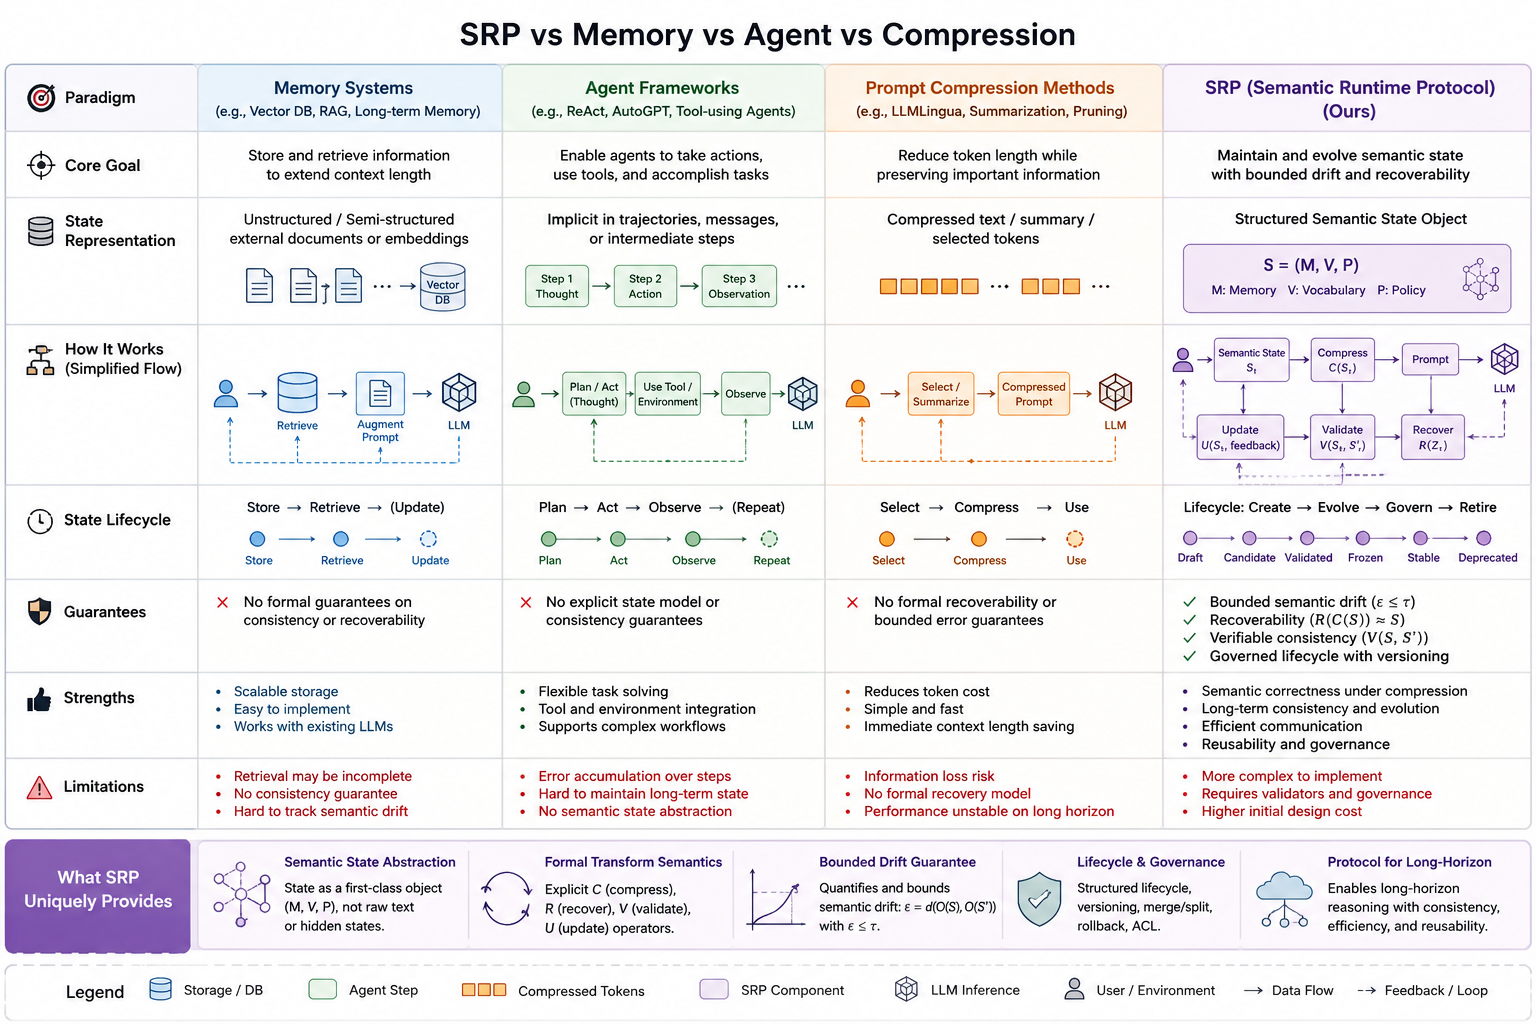
\includegraphics[width=0.9\linewidth]{../figures/SRP vs Memory vs Agent vs Compression.png}
  \caption{SRP as a semantic-state runtime layer between prompt/context management and downstream LLM reasoning.}
  \label{fig:positioning}
\end{figure}

\section{Related Work}
Research on long-horizon LLM systems has grown rapidly, but most existing approaches manage context indirectly through prompts, summaries, retrieval, or agent trajectories. SRP is related to these directions, but differs in its central claim: semantic state itself should be modeled as an explicit runtime object with governed transformation operators.

\subsection{Prompt Compression and Context Reduction}
One major line of work focuses on reducing prompt length while preserving task performance \citep{jiang2023llmlingua,liskavets2025cpc,jiang2024llmlingua2}. These methods show that raw prompt text often contains redundancy and can be shortened substantially without immediate loss in downstream utility.

However, prompt compression methods generally optimize prompts as token sequences rather than formalizing semantic state as a persistent computational object. Compression is typically a preprocessing step over context, not a runtime protocol with explicit recovery, validation, and update.

\subsection{Memory-Augmented LLM Systems}
Another major direction augments LLMs with external memory, including summary-based memory, episodic buffers, vector databases, and retrieval-augmented generation \citep{lewis2020rag,recursivelysummarizing2023,longmem2023,memorysurvey2025,cognitivememory2025}. These systems improve personalization and continuity by storing or retrieving prior information across turns.

Their limitation, for our purposes, is not lack of utility but lack of explicit transformation semantics. Summarization-based memory replaces earlier context with a lossy abstraction, while retrieval-based memory selects prior records without defining which semantic invariants should be preserved after reuse.

\subsection{Agent Frameworks and Trajectory-Based Systems}
Agent systems externalize long-horizon behavior through plans, tool calls, reasoning traces, and action trajectories. These systems are effective for structured task completion, but generally treat history as execution process rather than as a dedicated semantic state abstraction.

\subsection{Semantic Communication and Semantic Calibration}
SRP is also related to work on semantic communication, concept-level representation, and semantic calibration \citep{guo2024semanticnetworks,survey2025semanticcommunications,survey2025securesemantic}. These literatures motivate the shift from token fidelity to semantic fidelity and support the view that meaning preservation matters more than exact surface reproduction.

\subsection{Reproducibility, Replay, and LLM Evaluation}
Work on reproducibility, replay, prompt sensitivity, and experiment logging motivates the measurement side of SRP \citep{promptsensitivity2023,benchmarkingpromptsensitivity2025,assessingreproducibility2025,reproducibilityml2024,towardstrainingreproducible2022,reproducibilitygeneralizability2024}. Because semantic drift accumulates over multiple steps, replayable experiments and stable evaluation infrastructure are especially important.

\section{Runtime State and Operators}
We model the runtime state at interaction step $t$ as:
\begin{equation}
S_t = (M_t, V_t, P_t)
\end{equation}

where $M_t$ denotes structured semantic memory, $V_t$ denotes vocabulary state, and $P_t$ denotes the policy state governing transformation.

SRP defines four operators over semantic state:
\begin{align}
C &: S_t \to Z_t \\
R &: Z_t \to S_t' \\
\mathrm{Val} &: (S_t, S_t') \to [0,1] \\
U &: (S_t', F_t) \to S_{t+1}
\end{align}

Compression maps the current semantic state to a compact representation $Z_t$. Recovery reconstructs an operational state from that compact form. Validation estimates whether task-relevant meaning is preserved. Update revises the state based on recovered semantics and observed feedback.

\begin{figure}[t]
  \centering
  \fbox{\parbox{0.9\linewidth}{\centering Minimal SRP loop placeholder.}}
  \caption{Minimal SRP loop used in the semester-version experiment.}
  \label{fig:algorithm}
\end{figure}

\section{Formalization}
The purpose of the formalization is practical rather than philosophical. We do not attempt to prove semantic truth. Instead, we define measurable error over observable task behavior.

Let $O$ be a task-relevant observation operator that maps a semantic state to an observable behavior space:
\begin{equation}
O : S \to Y
\end{equation}

We define semantic error between original and recovered state as:
\begin{equation}
\epsilon(S, S') = d(O(S), O(S'))
\end{equation}

The goal is bounded degradation:
\begin{equation}
\epsilon(S, S') \le \tau
\end{equation}

Consider repeated transformation:
\begin{equation}
S_0 \xrightarrow{C} Z_0 \xrightarrow{R} S_1 \xrightarrow{C} Z_1 \xrightarrow{R} S_2 \to \cdots
\end{equation}

We define cumulative drift at step $k$ as:
\begin{equation}
\Delta_k = d(O(S_0), O(S_k))
\end{equation}

We say that an SRP instance satisfies bounded semantic drift over horizon $T$ if there exists a tolerance sequence $\{\tau_k\}$ such that for all $k \le T$:
\begin{equation}
\Delta_k \le \tau_k
\end{equation}

If each compression-recovery step incurs local error at most $e_t$, and the update operator magnifies incoming error by at most factor $\lambda$, then after $k$ cycles:
\begin{equation}
\Delta_k \le \sum_{i=0}^{k-1} \lambda^{k-1-i} e_i
\end{equation}

If $e_i \le e$ for all $i$, then:
\begin{equation}
\Delta_k \le e \sum_{i=0}^{k-1} \lambda^i
\end{equation}

This yields linear growth when $\lambda = 1$ and a finite geometric bound when $0 \le \lambda < 1$.

\subsection{Why Drift Is the Main Metric}

Drift is the primary metric because it is the shared failure mode across memory, retrieval, compression, and agent-based long-horizon systems. If repeated transformation is the operational setting, then drift is the most direct way to measure whether the semantic runtime abstraction is preserving task-relevant meaning over time.

In that sense, drift is not just one metric among several. It is the unifying quantity that the paper uses to compare systems across different context-management strategies.

\section{Experimental Setup}
We evaluate SRP in a finite-horizon setting designed to isolate bounded semantic drift under repeated transformation while keeping the study small enough to remain reproducible and interpretable. The goal is not to claim broad benchmark coverage, but to test whether explicit semantic-state management provides measurable stability benefits relative to lightweight baselines.

\subsection{Main Experimental Question}

The central experimental question is:

\begin{quote}
Does SRP maintain more stable task-relevant semantics over repeated compression-recovery cycles than lightweight baselines?
\end{quote}

\subsection{Main Methods}

The main comparison focuses on four methods: raw prompt, summarization, retrieval-based memory, and SRP.

\subsection{Main Tasks}

We use three task families: multi-turn instruction consistency, long-context summarization and regeneration, and iterative compression-recovery cycles.

\subsection{Benchmark and Replay}

To improve replicability, the paper should treat benchmark design and replayability as part of the contribution. A minimal benchmark is useful only if it can be replayed under the same prompt template, backend, model version, and evaluation settings. The repo therefore serves not only as implementation support, but also as a replayable record of the state transitions that the paper studies.

\begin{figure}[t]
  \centering
  \fbox{\parbox{0.9\linewidth}{\centering Drift over repeated compression-recovery cycles placeholder.}}
  \caption{Drift over repeated compression-recovery cycles.}
  \label{fig:drift}
\end{figure}

\begin{figure}[t]
  \centering
  \fbox{\parbox{0.9\linewidth}{\centering Token cost versus performance placeholder.}}
  \caption{Token cost versus performance for SRP and baselines.}
  \label{fig:tradeoff}
\end{figure}

\section{Results}
The semester version is designed to support a small number of clear empirical observations rather than a large benchmark sweep. The results section therefore prioritizes interpretability, reproducibility, and alignment with the paper's central claim.

\subsection{Drift Over Repeated Cycles}

The primary result is the semantic-drift-over-iterations analysis. This figure measures how quickly task-relevant semantic information degrades when each method is repeatedly subjected to compression-recovery cycles.

The main question is whether SRP exhibits a slower increase in cumulative semantic drift than lightweight baselines. If the SRP curve grows more slowly or remains flatter over the finite horizon, this would support the hypothesis that explicit semantic-state management may help stabilize repeated transformation.

\subsection{Quality and Task Preservation}

The second result concerns whether reduced drift corresponds to better preservation of task-relevant behavior. This is measured through task success under the selected core task families.

\subsection{Efficiency}

The third result concerns token cost. Since long-horizon systems are often constrained by context cost, the paper should evaluate whether SRP remains competitive in token usage while attempting to preserve semantic stability.

\subsection{Camera-Ready Comparison}

For a concise paper-facing view, the project also includes a camera-ready SRP versus strongest-baseline table. Its role is not to replace the fuller quality and efficiency analysis, but to provide a compact comparison that makes the central tradeoff immediately visible.

Under the current anchor-guided tuned local pilot, the clearest positive signal is that SRP now looks more balanced than plain summarization at `5` and `7` cycles, with higher task success and lower drift, even though retrieval-based memory still remains the strongest drift baseline on the present toy task suite.

\section{Discussion}
The main conceptual point of SRP is not that memory, retrieval, or agents are unnecessary. Rather, these components operate at adjacent layers. SRP targets the semantic-state layer itself.

\section{Limitations}
This work has several limitations. Drift is measured through proxies rather than direct semantic ground truth, results may depend on prompt design and judge model choice, and the current implementation uses a simplified version of SRP rather than the full blueprint.

\section{Open Questions To Preserve}
These should remain visible in the paper rather than being forced into a premature closure:

\begin{itemize}[leftmargin=*]
  \item Is SRP primarily a runtime abstraction, a protocol, or a semantic communication layer?
  \item What is the minimal semantic-state object?
  \item Which semantic drift metric should be considered the main one in the first paper?
  \item What failure cases should be shown explicitly?
\end{itemize}

\section{Future Work}
Several extensions are natural but should remain outside the first paper's main claim: richer semantic state schemas, stronger validator design, cross-model and cross-domain generalization, semantic package composition and conflict resolution, and replay databases.

\section{Conclusion}
We introduced SRP as a semantic-state runtime abstraction for long-horizon LLM interaction. The main takeaway is modest but important: long-horizon LLM stability may benefit from explicit semantic runtime design, and this hypothesis is concrete enough to formalize, implement, and test. The long-term vision remains broader, but the present paper is designed to answer one falsifiable question about this framework rather than many future-facing ones.

\section*{Acknowledgments}
This section is intentionally left blank for anonymous review. It can be filled in for a camera-ready version.

\appendix
\section{Additional Details}
The appendix can hold expanded proofs, additional experimental settings, ablations, or extra qualitative examples.

\bibliographystyle{plainnat}
\bibliography{references}

\end{document}
